\documentclass[11pt,titlepage]{article}

\usepackage{geometry}
\usepackage{float}
\usepackage{graphicx}
\geometry{a4paper}
\geometry{margin=2cm}
\geometry{portrait}

\newcommand{\horrule}[1]{\rule{\linewidth}{#1}}

\title{
		\normalfont \normalsize \textsc{Client Name: DVT} \\
		\normalfont \normalsize \textsc{Project Name: KinderFinder} \\ [25pt]
		\horrule{0.5pt} \\[0.4cm]
		\huge Vision and Scope Document \\
		\horrule{2pt} \\[0.5cm]
}
\author{\begin{tabular}{r l}
	\texttt{Team Name:} & \texttt{MAU Technologies} \\[0.5cm]
	Uteshlen Nadesan & 28163304 \\
	Michael Johnston & 12053300 \\
	Po-Han Chiu & 11063612
\end{tabular}
	\\ \\ \texttt{https://github.com/MrBean355/KinderFinder.git}
	\\ \\ \texttt{Version: 0.1}}
\date{1 August 2014} 

\begin{document}
\maketitle
\tableofcontents
\newpage

\section{Introduction}
This document was developed at the beginning of the project, but is to be constantly adapted as the vision and scope evolve.\\
The system will consist of five main components, namely:
\begin{itemize}
\item Web Administration
\item Mobile Application (Android)
\item Web API
\item Reporting
\item Embedded Hardware and Prototyping
\end{itemize}

\section{Scope and Limitations}
The system will track children throughout a specific area (for example, in a restaurant). The children will be wearing some kind of wristband which contains RFID technology that will relay the position to receivers. The position will be overlayed onto a map which is viewed by parents on their mobile devices. The system is to maintain its own database to store the necessary data.\\
Embedded Hardware and Prototyping is mainly a proof of concept (POC) component. The software side of the system is to be focused on during development and the hardware will be incorporated if time allows.\\
An extension in the future, but is out of scope for the project, is a device that is placed on the diners' table that lights up according to which zone the child is currently in.\\
There will be a basic reporting module, available through the web portal to system administrators. It will provide statistics such as which zones are used the most, how often specific customers use the service and whether any of the hardware devices are broken or malfunctioning.
\subsection{Use Cases}
\begin{figure}[H]
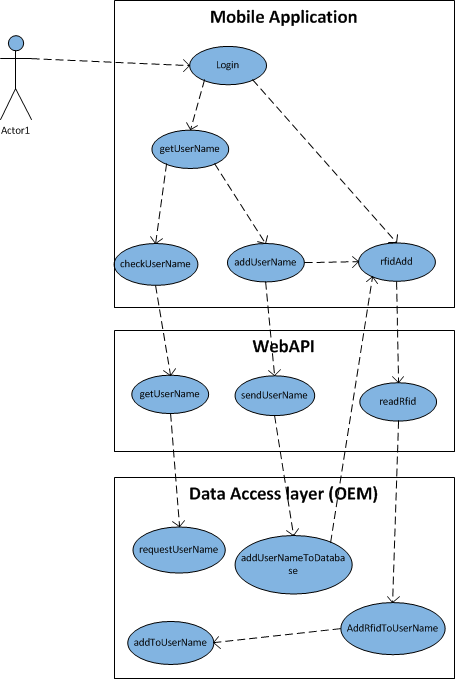
\includegraphics[scale=1.0]{UseCaseLogin.png}
\caption{Log in and add RFID use cases.}
\end{figure}
\begin{figure}[H]
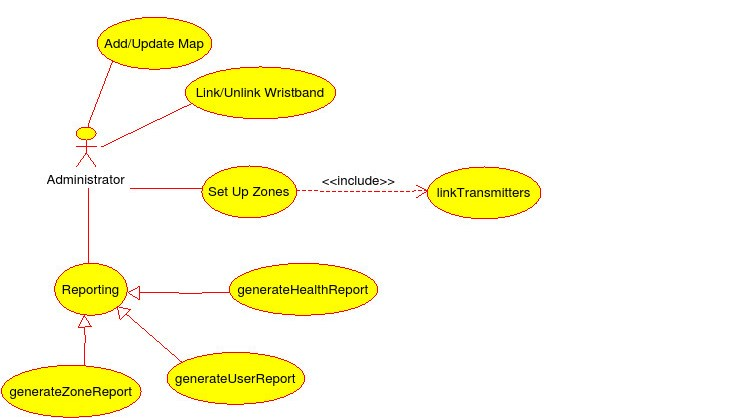
\includegraphics[scale=0.9]{UseCase2.jpg}
\caption{Locate child and administration use cases.}
\end{figure}
\end{document}
